\section{Experiments}
\label{sec:experiments_007}

In this section, we compare \NatPNacro{} to existing methods on extensive experiments including three different tasks: classification, regression and count prediction. For each task type, we evaluate the prediction quality based on target error and uncertainty metrics. These various set-ups aim to highlight the versatility of \NatPNacro{}. In particular, \NatPNacro{} is the only model that adapts to all tasks and achieves high performances for all metrics without requiring multiple forward passes.

\begin{table*}[ht]
    \centering
    % \vspace{-1mm}
   % \scriptsize
   \caption{Classification results on Sensorless Drive with Categorical target distribution. Best scores among all single-pass models are in bold. Best scores among all models are starred.}
    \label{tab:sensorless-drive}
    % \vspace{-3mm}
    \resizebox{0.8 \textwidth}{!}{
    \begin{tabular}{lcccccc}
        \toprule
        & \textbf{Accuracy} & \textbf{Brier} & \textbf{9/10 Alea.} & \textbf{9/10 Epist.} & \textbf{OODom Alea.} & \textbf{OODom Epist.} \\
        \midrule
        \textbf{Dropout} & 98.62 $\pm$ 0.11 & 3.79 $\pm$ 0.29 & 30.20 $\pm$ 0.85 & 32.57 $\pm$ 1.45 & 27.03 $\pm$ 0.51 & 95.30 $\pm$ 1.66 \\
        \textbf{Ensemble} & 98.83 $\pm$ 0.17 & 3.00 $\pm$ 0.54 & 30.79 $\pm$ 0.74 & 32.61 $\pm$ 1.06 & 27.16 $\pm$ 0.59 & 99.97 $\pm$ 0.01 \\
        \textbf{NatPE} & *99.66 $\pm$ 0.03 & *0.68 $\pm$ 0.05 & 77.05 $\pm$ 1.93 & 83.73 $\pm$ 1.89 & 99.99 $\pm$ 0.00 & *100.00 $\pm$ 0.00 \\
        \midrule
        \textbf{R-PriorNet} & 98.85 $\pm$ 0.25 & 2.01 $\pm$ 0.47 & 40.13 $\pm$ 2.99 & 30.07 $\pm$ 0.81 & \textbf{*100.00 $\pm$ 0.00} & 23.59 $\pm$ 0.00 \\
        \textbf{EnD$^2$} & 93.95 $\pm$ 2.35 & 28.09 $\pm$ 6.40 & 26.35 $\pm$ 0.60 & 24.85 $\pm$ 0.43 & 84.43 $\pm$ 15.21 & 23.58 $\pm$ 0.00 \\
        \textbf{PostNet} & \textbf{99.64 $\pm$ 0.02} & \textbf{0.75 $\pm$ 0.08} & 80.60 $\pm$ 1.68 & \textbf{*92.57 $\pm$ 1.41} & \textbf{*100.00 $\pm$ 0.00} & \textbf{*100.00 $\pm$ 0.00} \\
        \textbf{\NatPNacro{}} & 99.61 $\pm$ 0.05 & 1.04 $\pm$ 0.29 & \textbf{*81.43 $\pm$ 1.89} & 79.54 $\pm$ 2.62 & 99.98 $\pm$ 0.00 & \textbf{*100.00 $\pm$ 0.00} \\
        \bottomrule
    \end{tabular}
    }
            % \vspace{-0mm}
\end{table*}

%\begin{table*}[ht]
%    \centering
%    \scriptsize
%    \resizebox{1.\textwidth}{!}{
%    \begin{tabular}{lcccccccc}
%        \toprule
%        & \textbf{Accuracy} & \textbf{Brier} & \textbf{K. Alea.} & \textbf{K. Epist.} & \textbf{F. Alea.} & \textbf{F. Epist.} & \textbf{OODom Alea.} & \textbf{OODom Epist.} \\
%        \midrule
%        \textbf{Dropout} & 99.45 $\pm$ 0.01 & 1.07 $\pm$ 0.05 & 98.27 $\pm$ 0.05 & 97.82 $\pm$ 0.08 & *99.40 $\pm$ 0.03 & 98.01 $\pm$ 0.14 & 43.86 $\pm$ 1.62 & 74.09 $\pm$ 0.92 \\
%        \textbf{Ensemble} & 99.46 $\pm$ 0.02 & 1.02 $\pm$ 0.02 & 98.39 $\pm$ 0.07 & 98.43 $\pm$ 0.05 & 99.33 $\pm$ 0.06 & 98.73 $\pm$ 0.08 & 40.98 $\pm$ 1.80 & 66.54 $\pm$ 0.58 \\
%        \textbf{NatPE} & *99.55 $\pm$ 0.01 & *0.84 $\pm$ 0.03 & 96.39 $\pm$ 0.73 & *99.61 $\pm$ 0.02 & 97.49 $\pm$ 0.85 & *99.70 $\pm$ 0.04 & *100.00 $\pm$ 0.00 & *100.00 $\pm$ 0.00 \\
%        \midrule
%        \textbf{R-PriorNet} & 99.35 $\pm$ 0.04 & \textbf{0.97 $\pm$ 0.03} & \textbf{*99.33 $\pm$ 0.18} & 99.28 $\pm$ 0.25 & \textcolor{gray}{100.00 $\pm$ 0.00} & \textcolor{gray}{100.00 $\pm$ 0.00} & 97.48 $\pm$ 0.66 & 31.03 $\pm$ 0.13 \\
%        \textbf{EnD$^2$} & 99.24 $\pm$ 0.05 & 6.19 $\pm$ 0.13 & 98.36 $\pm$ 0.15 & 98.76 $\pm$ 0.13 & \textbf{99.25 $\pm$ 0.16} & 99.35 $\pm$ 0.14 & 48.09 $\pm$ 1.38 & 31.60 $\pm$ 0.39 \\
%        \textbf{PostNet} & 99.36 $\pm$ 0.02 & 1.33 $\pm$ 0.04 & 98.88 $\pm$ 0.05 & 98.79 $\pm$ 0.07 & 98.89 $\pm$ 0.23 & 98.85 $\pm$ 0.23 & \textbf{*100.00 $\pm$ 0.00} & \textbf{*100.00 $\pm$ 0.00} \\
%        \textbf{\NatPNacro{}} & \textbf{99.47 $\pm$ 0.02} & 1.09 $\pm$ 0.03 & 99.20 $\pm$ 0.20 & \textbf{99.39 $\pm$ 0.08} & 99.16 $\pm$ 0.28 & \textbf{99.54 $\pm$ 0.09} & 99.99 $\pm$ 0.01 & \textbf{*100.00 $\pm$ 0.00} \\
%        \bottomrule
%    \end{tabular}
%    }
%    \caption{Results on MNIST (classification with Categorical target distribution). Best scores among all single-pass models are in bold. Best scores among all models are starred. Gray numbers indicate that R-PriorNet has seen samples from the FMNIST dataset during training.}
%    \label{tab:mnist}
            %\vspace{-.3cm}
%\end{table*}

%\begin{table*}[ht]
% \centering
% \scriptsize
% \resizebox{\textwidth}{!}{
% \begin{tabular}{lcccccccc}
%     \toprule
%     & \textbf{Accuracy} & \textbf{Brier} & \textbf{M. Alea.} & \textbf{M. Epist.} & \textbf{K. Alea.} & \textbf{K. Epist.} & \textbf{OODom Alea.} & \textbf{OODom Epist.} \\
%     \midrule
%     \textbf{Dropout} & 92.44 $\pm$ 0.17 & 13.89 $\pm$ 0.31 & 60.75 $\pm$ 1.41 & 75.85 $\pm$ 1.73 & 76.57 $\pm$ 1.30 & 92.48 $\pm$ 0.46 & 39.97 $\pm$ 0.69 & 90.90 $\pm$ 1.74 \\
%     \textbf{Ensemble} & 92.64 $\pm$ 0.10 & 13.63 $\pm$ 0.25 & 77.14 $\pm$ 1.49 & 90.78 $\pm$ 0.75 & 86.20 $\pm$ 0.76 & 95.16 $\pm$ 0.35 & 37.30 $\pm$ 0.83 & 82.93 $\pm$ 0.96 \\
%     \textbf{NatPE} & *92.89 $\pm$ 0.06 & 14.44 $\pm$ 0.06 & 82.56 $\pm$ 0.33 & 96.38 $\pm$ 0.29 & 92.12 $\pm$ 0.17 & *98.79 $\pm$ 0.09 & *100.00 $\pm$ 0.00 & *100.00 $\pm$ 0.00 \\
%     \midrule
%     \textbf{R-PriorNet} & 91.53 $\pm$ 0.10 & \textbf{*12.21 $\pm$ 0.20} & \textbf{*98.83 $\pm$ 0.49} & \textbf{*99.54 $\pm$ 0.18} & \textcolor{gray}{99.96 $\pm$ 0.02} & \textcolor{gray}{99.99 $\pm$ 0.00} & 72.23 $\pm$ 6.32 & 48.84 $\pm$ 6.09 \\
%     \textbf{EnD$^2$} & \textbf{91.84 $\pm$ 0.03} & 29.23 $\pm$ 0.79 & 79.32 $\pm$ 1.39 & 91.61 $\pm$ 1.04 & 91.99 $\pm$ 0.06 & 98.36 $\pm$ 0.20 & 43.70 $\pm$ 3.37 & 36.73 $\pm$ 3.74 \\
%     \textbf{PostNet} & 91.04 $\pm$ 0.10 & 16.11 $\pm$ 0.30 & 90.56 $\pm$ 1.25 & 92.10 $\pm$ 1.77 & \textbf{*96.65 $\pm$ 0.33} & 97.06 $\pm$ 0.42 & \textbf{*100.00 $\pm$ 0.00} & \textbf{*100.00 $\pm$ 0.00} \\
%     \textbf{\NatPNacro{}} & 91.65 $\pm$ 0.14 & 14.88 $\pm$ 0.30 & 81.12 $\pm$ 2.77 & 96.51 $\pm$ 0.81 & 93.03 $\pm$ 1.00 & \textbf{98.38 $\pm$ 0.23} & 99.99 $\pm$ 0.01 & \textbf{*100.00 $\pm$ 0.00} \\
%     \bottomrule
% \end{tabular}
% }
% \caption{Results on FMNIST (classification with Categorical target distribution). Best scores among all single-pass models are in bold. Best scores among all models are starred. Gray numbers indicate that R-PriorNet has seen samples from the KMNIST dataset during training.}
% \label{tab:fmnist}
%\end{table*}

\begin{table*}[ht]
    \centering
    	% \vspace{-4mm}
    %\scriptsize
    \caption{Classification results on CIFAR-10 with Categorical target distribution. Best scores among all single-pass models are in bold. Best scores among all models are starred. Gray numbers indicate that R-PriorNet has seen samples from the SVHN dataset during training.}
    % \vspace{-3mm}
    \resizebox{.9\textwidth}{!}{
    \begin{tabular}{lcccccccc}
        \toprule
        & \textbf{Accuracy} & \textbf{Brier} & \textbf{SVHN Alea.} & \textbf{SVHN Epist.} & \textbf{CelebA Alea.} & \textbf{CelebA Epist.} & \textbf{OODom Alea.} & \textbf{OODom Epist.} \\
        \midrule
        \textbf{Dropout} & 88.15 $\pm$ 0.20 & 19.59 $\pm$ 0.41 & 80.63 $\pm$ 1.59 & 73.09 $\pm$ 1.51 & 71.84 $\pm$ 4.28 & 71.04 $\pm$ 3.92 & 18.42 $\pm$ 1.11 & 49.69 $\pm$ 9.10 \\
        \textbf{Ensemble} & *89.95 $\pm$ 0.11 & 17.33 $\pm$ 0.17 & 85.26 $\pm$ 0.84 & 82.51 $\pm$ 0.63 & 76.20 $\pm$ 0.87 & 74.23 $\pm$ 0.78 & 25.30 $\pm$ 4.02 & 89.21 $\pm$ 7.55 \\
        \textbf{NatPE} & 89.21 $\pm$ 0.09 & 17.41 $\pm$ 0.12 & 85.66 $\pm$ 0.34 & *83.16 $\pm$ 0.67 & *78.95 $\pm$ 1.15 & *82.06 $\pm$ 1.30 & 87.27 $\pm$ 1.79 & *98.88 $\pm$ 0.26 \\
        \midrule
        \textbf{R-PriorNet} & \textbf{88.94 $\pm$ 0.23} & \textbf{*15.99 $\pm$ 0.32} & \textcolor{gray}{99.87 $\pm$ 0.02} & \textcolor{gray}{99.94 $\pm$ 0.01} & 67.74 $\pm$ 4.86 & 59.55 $\pm$ 7.90 & 42.21 $\pm$ 8.77 & 38.25 $\pm$ 9.82 \\
        \textbf{EnD$^2$} & 84.03 $\pm$ 0.25 & 40.84 $\pm$ 0.36 & \textbf{*86.47 $\pm$ 0.66} & \textbf{81.84 $\pm$ 0.92} & 75.54 $\pm$ 1.79 & 75.94 $\pm$ 1.82 & 42.19 $\pm$ 8.77 & 15.79 $\pm$ 0.27 \\
        %\textbf{SNGP} & 79.40 $\pm$ 0.96 & 38.76 $\pm$ 1.61 & 71.65 $\pm$ 0.89 & -- & 72.46 $\pm$ 2.23 & -- & 83.35 $\pm$ 5.93 & -- \\
        \textbf{PostNet} & 87.95 $\pm$ 0.20 & 20.19 $\pm$ 0.40 & 82.35 $\pm$ 0.68 & 79.24 $\pm$ 1.49 & 72.96 $\pm$ 2.33 & 75.84 $\pm$ 1.61 & 85.89 $\pm$ 4.10 & 92.30 $\pm$ 2.18 \\
        \textbf{\NatPNacro{}} & 87.90 $\pm$ 0.16 & 19.99 $\pm$ 0.46 & 82.29 $\pm$ 1.11 & 77.83 $\pm$ 1.22 & \textbf{76.01 $\pm$ 1.18} & \textbf{76.87 $\pm$ 3.38} & \textbf{*93.67 $\pm$ 3.03} & \textbf{94.90 $\pm$ 3.09} \\
        \bottomrule
    \end{tabular}
    }
    \label{tab:cifar10}
            % \vspace{-4mm}
\end{table*}

\begin{table*}[ht]
    \centering
    %\scriptsize
        \caption{Results on the Bike Sharing Dataset with Normal $\DNormal$ and Poison $\DPoi$ target distributions. Best scores among all single-pass models are in bold. Best scores among all models are starred.}
    \label{tab:bike-sharing}
    % \vspace{-3mm}
    \resizebox{0.9\textwidth}{!}{
    \begin{tabular}{lcccccc}
        \toprule
        & \textbf{RMSE} & \textbf{Calibration} & \textbf{Winter Epist.} & \textbf{Spring Epist.} & \textbf{Autumn Epist.} & \textbf{OODom Epist.} \\
        \midrule
        \textbf{Dropout-$\DNormal$} & 70.20 $\pm$ 1.30 & 6.05 $\pm$ 0.77 & 15.26 $\pm$ 0.51 & 13.66 $\pm$ 0.16 & 15.11 $\pm$ 0.46 & 99.99 $\pm$ 0.01 \\
        \textbf{Ensemble-$\DNormal$} & *48.02 $\pm$ 2.78 & 5.88 $\pm$ 1.00 & 42.46 $\pm$ 2.29 & 21.28 $\pm$ 0.38 & 21.97 $\pm$ 0.58 & *100.00 $\pm$ 0.00 \\
        \midrule
        \textbf{EvReg-$\DNormal$} & \textbf{49.58 $\pm$ 1.51} & 3.77 $\pm$ 0.81 & 17.19 $\pm$ 0.76 & 15.54 $\pm$ 0.65 & 14.75 $\pm$ 0.29 & 34.99 $\pm$ 17.02 \\
        \textbf{\NatPNacro{}-$\DNormal$} & 49.85 $\pm$ 1.38 & \textbf{*1.95 $\pm$ 0.34} & \textbf{*55.04 $\pm$ 6.81} & \textbf{*23.25 $\pm$ 1.20} & \textbf{*27.78 $\pm$ 2.47} & \textbf{*100.00 $\pm$ 0.00} \\
        \midrule
        \midrule
        \textbf{Dropout-$\DPoi$} & 66.57 $\pm$ 4.61 & 55.00 $\pm$ 0.22 & 16.02 $\pm$ 0.48 & 13.48 $\pm$ 0.38 & 18.09 $\pm$ 0.82 & \textbf{*100.00 $\pm$ 0.00} \\
        \textbf{Ensemble-$\DPoi$} & \textbf{*48.22 $\pm$ 2.06} & 55.31 $\pm$ 0.21 & 83.88 $\pm$ 1.22 & 34.21 $\pm$ 1.81 & 41.29 $\pm$ 3.23 & \textbf{*100.00 $\pm$ 0.00} \\
        \midrule
        \textbf{\NatPNacro{}-$\DPoi$} & 51.79 $\pm$ 0.78 & \textbf{*31.04 $\pm$ 1.81} & \textbf{*85.15 $\pm$ 3.61} & \textbf{*37.03 $\pm$ 2.35} & \textbf{*42.73 $\pm$ 4.38} & \textbf{*100.00 $\pm$ 0.00} \\
        \bottomrule
    \end{tabular}
    }
            % \vspace{-3mm}
\end{table*}

\begin{table*}[t]
    \centering
   % \scriptsize
   \caption{Regression results on models trained on different UCI datasets with Normal target distribution. The upper half displays models trained on Kin8nm, the lower half shows models trained on Concrete Compressive Strength.}
    \label{tab:uci}
    % \vspace{-3mm}
    \resizebox{1.\textwidth}{!}{
    \begin{tabular}{lcccccccc}
        \toprule
        & \textbf{RMSE} & \textbf{Calibration} & \textbf{Energy Alea.} & \textbf{Energy Epist.} & \textbf{Concrete Alea.} & \textbf{Concrete Epist.} & \textbf{Kin8nm Alea.} & \textbf{Kin8nm Epist.} \\
        \midrule
        \textbf{Dropout} & 0.09 $\pm$ 0.00 & 3.13 $\pm$ 0.43 & 90.18 $\pm$ 6.00 & 99.94 $\pm$ 0.06 & *100.00 $\pm$ 0.00 & *100.00 $\pm$ 0.00 & \multicolumn{2}{c}{\multirow{3}{*}{\textbf{in-distribution}}} \\
        \textbf{Ensemble} & *0.07 $\pm$ 0.00 & 2.69 $\pm$ 0.49 & *100.00 $\pm$ 0.00 & *100.00 $\pm$ 0.00 & *100.00 $\pm$ 0.00 & *100.00 $\pm$ 0.00 & & \\
        \textbf{NatPE} & 0.08 $\pm$ 0.00 & 5.49 $\pm$ 0.30 & *100.00 $\pm$ 0.00 & *100.00 $\pm$ 0.00 & *100.00 $\pm$ 0.00 & *100.00 $\pm$ 0.00 & & \\
        \midrule
        \textbf{EvReg} & 0.09 $\pm$ 0.00 & 3.74 $\pm$ 0.53 & 88.06 $\pm$ 11.94 & 88.06 $\pm$ 11.94 & \textbf{*100.00 $\pm$ 0.00} & 86.84 $\pm$ 13.16 & \multicolumn{2}{c}{\multirow{2}{*}{\textbf{in-distribution}}} \\
        \textbf{\NatPNacro{}} & \textbf{0.08 $\pm$ 0.00} & \textbf{*2.04 $\pm$ 0.45} & \textbf{*100.00 $\pm$ 0.00} & \textbf{*100.00 $\pm$ 0.00} & \textbf{*100.00 $\pm$ 0.00} & \textbf{*100.00 $\pm$ 0.00} & & \\
        \midrule
        \midrule
        \textbf{Dropout} & 5.67 $\pm$ 0.07 & *3.03 $\pm$ 0.40 & 9.33 $\pm$ 0.36 & 93.53 $\pm$ 2.41 & \multicolumn{2}{c}{\multirow{3}{*}{\textbf{in-distribution}}} & 1.09 $\pm$ 0.13 & 64.30 $\pm$ 7.14 \\
        \textbf{Ensemble} & 5.69 $\pm$ 0.20 & 3.81 $\pm$ 0.67 & 54.19 $\pm$ 18.93 & *100.00 $\pm$ 0.00 & & & 72.57 $\pm$ 19.32 & *100.00 $\pm$ 0.00 \\
        \textbf{NatPE} & *4.78 $\pm$ 0.20 & 5.58 $\pm$ 1.27 & *100.00 $\pm$ 0.00 & *100.00 $\pm$ 0.00 & & & *100.00 $\pm$ 0.00 & *100.00 $\pm$ 0.00 \\
        \midrule
        \textbf{EvReg} & 6.04 $\pm$ 0.18 & 7.36 $\pm$ 1.04 & 8.93 $\pm$ 0.02 & 51.39 $\pm$ 18.56 & \multicolumn{2}{c}{\multirow{2}{*}{\textbf{in-distribution}}} & 0.93 $\pm$ 0.00 & 34.44 $\pm$ 20.95 \\
        \textbf{\NatPNacro{}} & \textbf{5.83 $\pm$ 0.23} & \textbf{5.41 $\pm$ 1.33} & \textbf{*100.00 $\pm$ 0.00} & \textbf{*100.00 $\pm$ 0.00} & & & \textbf{*100.00 $\pm$ 0.00} & \textbf{*100.00 $\pm$ 0.00} \\
        \bottomrule
    \end{tabular}}
    % \vspace{-4mm}
\end{table*}

\begin{table*}[t]
    \centering
 %   \scriptsize
     \caption{Regression results on NYU Depth v2 with Normal target distribution. RMSE is in cm. OOD scores on LSUN are reported on the held-out classes `classrooms' (left) and `churches' (right).}
    \label{tab:nyu}
    \vspace{-0mm}
    \resizebox{1. \textwidth}{!}{
    \begin{tabular}{lcccccccccc}
        \toprule
        & \textbf{RMSE} & \textbf{Calibration} & \textbf{LSUN Alea.} & \textbf{LSUN Epist.} & \textbf{KITTI Alea.} & \textbf{KITTI Epist.} & \textbf{OODom Alea.} & \textbf{OODom Epist.} \\
        \midrule
        \textbf{Dropout} & 46.95 & 4.03 & *95.29 / 97.74 & 83.89 / 83.22 & 98.07 & 84.90 & 74.40 & *100.00 \\
        \midrule
        \textbf{EvReg} & \textbf{*28.88} & \textbf{*1.05} & 58.70 / 56.71 & 70.19 / 64.02 & 56.60 & 62.67 & 75.43 & 56.39 \\
        \textbf{\NatPNacro{}} & 29.72 & 1.14 & \textbf{94.13} / \textbf{*98.67} & \textbf{*89.08} / \textbf{*90.56} & \textbf{*98.93} & \textbf{*93.15} & \textbf{*100.00} & \textbf{*100.00} \\
        \bottomrule
    \end{tabular}}
    \vspace{-0mm}
\end{table*}

\subsection{Setup}

% \begin{wrapfigure}{r}{0.5\textwidth}
\begin{figure*}[t]
\vspace{-4mm}
	\centering
    \includegraphics[width=.8\linewidth]{sections/007_iclr2022/resources/corruptions-final-crop.pdf}
    \caption{Averaged accuracy and confidence under 15 dataset shifts on CIFAR-10 \citep{benchmarking-corruptions}. 
    On more severe perturbations (i.e. data further away from data distribution), \NatPNacro{} maintains a competitive accuracy while assigning higher epistemic uncertainty as desired. Baselines provide a slower relative confidence decay.
    }
    \label{fig:data-corruption}
\vspace{-4mm}
\end{figure*}
% \end{wrapfigure}

In our experiments, we change the encoder architecture of \NatPNacro{} to match the dataset needs. We perform a grid search over normalizing flows types (i.e. radial flows \citep{radialflow} and MAF \citep{made,maf}) and latent dimensions. We show further experiments on architecture, latent dimension, normalizing flow choices and certainty budget choice in the appendix. Furthermore, we use approximations of the log-Gamma $\log\Gamma(x)$ and the Digamma $\psi(x)$ functions for large input values to avoid unstable floating computations (see app.). As prior parameters, we set ${\bm{\chi}^\text{prior}=\bm{1}_{\nclass}/C}, {\evidence^\text{prior}=\nclass}$ for classification, ${\priorparam^\text{prior}=(0, 100)^T}, \evidence^\text{prior}=1$ for regression and $\chi^\text{prior}=1, \evidence^\text{prior}=1$ for count prediction enforcing high entropy for prior distributions.

\paragraph{Baselines.} We focus on recent models parametrizing prior distributions over the target distribution. For classification, we compare \NatPNacro{} to Reverse KL divergence Prior Networks (R-PriorNet) \citep{reverse-kl}, Ensemble Distribution Distillation (EnD$^2$) \citep{distribution-distillation} and Posterior Networks (PostNet) \citep{charpentier2020}. Note that Prior Networks require OOD training data --- we use an auxiliary dataset when available and Gaussian noise otherwise. For regression, we compare to Evidential Regression (EvReg) \citep{evidential-regression}. Beyond baselines parametrizing conjugate prior distributions, we also compare to dropout (Dropout) \citep{dropout} and ensemble (Ensemble) \citep{ensembles} models for all tasks. These sampling baselines require multiple forward passes for uncertainty estimation. 
Further details are given in the appendix.
%As suggested in \citep{dataset-shift}, we use $5$ samples for the two sampling baselines. Note that, unlike the other baselines or \NatPNacro{}, the sampling baselines require multiple forward passes for uncertainty estimation. 
%In all experiments, all models share the same backbone architecture (MLP, Conv. \citep{conv-net}, DenseDepth \citep{dense-depth}). We use early stopping and perform a grid search on the hyperparameters of all models including learning rate, dropout rate and regularizing factor when applicable. We report average results over $5$ initialization seeds with standard error of the mean (except for the larger dataset NYU Depth v2 dataset). Further model details are given in the appendix.


%\textbf{Baselines.} We focus on recent models parametrizing prior distributions over the target distribution. For classification, we compare \NatPNacro{} to Reverse KL divergence Prior Networks \textbf{(R-PriorNet)} \citep{reverse-kl}, Ensemble Distribution Distillation \textbf{(EnD$^2$)} \citep{distribution-distillation} and Posterior Networks \textbf{(PostNet)} \citep{charpentier2020}. Note that Prior Networks require OOD training data --- we use an auxiliary dataset when available and Gaussian noise otherwise. For regression, we compare to Evidential Regression \textbf{(EvReg)} \citep{evidential-regression}. Beyond baselines parametrizing conjugate prior distributions, we also compare to dropout \textbf{(Dropout)} \citep{dropout} and ensemble \textbf{(Ensemble)} \citep{ensembles} models for all tasks. As suggested in \citep{dataset-shift}, we use $5$ samples for the two sampling baselines. Note that, unlike the other baselines or \NatPNacro{}, the sampling baselines require multiple forward passes for uncertainty estimation. 
%In all experiments, all models share the same backbone architecture (MLP, Conv. \citep{conv-net}, DenseDepth \citep{dense-depth}). We use early stopping and perform a grid search on the hyperparameters of all models including learning rate, dropout rate and regularizing factor when applicable. We report average results over $5$ initialization seeds with standard error of the mean (except for the larger dataset NYU Depth v2 dataset). Further model details are given in the appendix.

\paragraph{Datasets.} We split all datasets into train, validation and test sets. For classification, we use one tabular dataset (Sensorless Drive \citep{uci_datasets}) and three image datasets (MNIST \citep{mnist}, FMNIST \citep{fashionmnist} and CIFAR-10 \citep{cifar10}). For count prediction, we use the Bike Sharing dataset \citep{bike-sharing} to predict the number of bike rentals within an hour. For regression, we also use the Bike Sharing dataset where the target is viewed as continuous, real-world UCI datasets used in \citep{evidential-regression, probabilistic-backprop-scalable-bnn} and the image NYU Depth v2 dataset \citep{nyu-depth} where the goal is to predict the image depth per pixel. All inputs are rescaled with zero mean and unit variance. We also scale the output target for regression. Further details are given in the appendix.

\paragraph{Metrics.} Beyond the target prediction error, we evaluate model uncertainty estimation using calibration and OOD detection scores. Furthermore, we report the inference speed. Further results including histograms with uncertainty estimates or latent space visualization are presented in appendix. 

\textit{\underline{Target error:}} We use the accuracy (Accuracy) for classification and the Root Mean Squared Error (RMSE) for regression and count prediction. 

\textit{\underline{Calibration:}} For classification, we use the Brier score (Brier) \citep{scoring-rules}. For regression and count prediction, we use the quantile calibration score (Calibration) \citep{accurate-uncertainties-deep-learning-regression}. 

\textit{\underline{OOD detection:}} We evaluate how the uncertainty scores enable to detect OOD data using the area under the precision-recall curve (AUC-PR) the area under the receiver operating characteristic curve (AUC-ROC) in the appendix. We use two different uncertainty measures: the negative entropy of the predicted target distribution accounting for the aleatoric uncertainty (Alea. OOD) and the predicted evidence or variance of the predicted mean (Epist. OOD). Similarly to \citep{dataset-shift, charpentier2020}, we use four different types of clear OOD samples: Unseen datasets (KMNIST \cite{kmnist}, Fashion-MNIST \citep{fashionmnist}, SVHN \citep{svhn}, LSUN \citep{lsun}, CelebA \citep{celeba}, KITTI \citep{kitti}), left-out data (classes 9/10 for Sensorless Drive, winter/spring/autumn seasons for Bike Sharing), out-of-domain data not normalized in $[0, 1]$ (OODom) and dataset shifts (corrupted CIFAR-10 \citep{benchmarking-corruptions}). Further details are given in the appendix.

%\textbf{Metrics.} Beyond the target prediction error, we evaluate model uncertainty estimation using calibration and OOD detection scores. Furthermore, we report the inference speed. Further results including histograms with uncertainty estimates or latent space visualization are presented in appendix. \textit{\underline{Target error:}} We use the accuracy \textbf{(Accuracy)} for classification and the Root Mean Squared Error \textbf{(RMSE)} for regression and count prediction. \textit{\underline{Calibration:}} Calibration scores aim at evaluating if the error from the predicted target distribution corresponds to the empirical error achieved by the model (e.g. is a class prediction with a predicted confidence $p_\iclass=80\%$ correct $80\%$ of the time?). For classification, we use the Brier score \textbf{(Brier)} \citep{scoring-rules}. For regression and count prediction, we use the absolute difference between the percentile $p$ and the percentage $p_\text{pred}$ of target lying in the confidence interval $I_p=[0,\frac{p}{2}]\cup[1-\frac{p}{2},1]$ under the predicted target distribution. We compute a single calibration score by summing the square difference for $p \in \{0.1, \ldots, 0.9\}$ i.e.  \smash{$\sqrt{\sum_p (p - p_\text{pred})^2}$} \textbf{(Calibration)} \citep{accurate-uncertainties-deep-learning-regression}. \textit{\underline{OOD detection:}} We evaluate how the uncertainty scores enable to detect OOD data using the area under the precision-recall curve (AUC-PR). We show further results using the area under the receiver operating characteristic curve (AUC-ROC) in appendix. We use two different uncertainty measures: the negative entropy of the predicted target distribution accounting for the aleatoric uncertainty \textbf{(Alea. OOD)} and the predicted evidence \textbf{(Epist. OOD)}. Similarly to \citep{dataset-shift, postnet, reverse-kl}, we use four different types of clear OOD samples: Unseen datasets (KMNIST \cite{kmnist}, Fashion-MNIST \citep{fashion-mnist}, SVHN \citep{svhn}, LSUN \citep{lsun}, CelebA \citep{celeba}, KITTI \citep{kitti}), left-out data (classes 9/10 for Sensorless Drive, winter/spring/autumn seasons for Bike Sharing), out-of-domain data not normalized in $[0, 1]$ (\textbf{OODom}) and dataset shifts (corrupted CIFAR-10 \citep{benchmarking-corruptions}).

\subsection{Results}

\paragraph{Classification.} We show results for the tabular dataset Sensorless Drive with unbounded input domain in Tab.~\ref{tab:sensorless-drive}, and the image datasets MNIST, FMNIST and CIFAR-10 with bounded input domain in Tab.~\ref{tab:cifar10} and appendix. Overall, for classification \NatPNacro{} performs on par with best single-pass baselines (i.e. $12/30$ top-1 scores, $25/30$ top-2 scores) and NatPE performs the best among multiple-pass models (i.e. $28/30$ top-1 scores). A single \NatPNacro{} achieves accuracy and calibration performance on par with the most calibrated baselines, namely PostNet and R-PriorNet which requires one normalizing flow per class or training OOD data. Further, NatPE consistently improves accuracy and calibration performance of a single \NatPNacro{} which underlines the benefit of aggregating multiple models predictions for accuracy and calibration \citep{ensembles}. Without requiring OOD data during training, both \NatPNacro{} and NatPE achieve excellent OOD detection scores w.r.t. all OOD types. This strongly suggests that \NatPNacro{} does \emph{not} suffer from the flaws in \cite{anomaly-detection,deep-generative,typicality_OOD_generative}. In particular, \NatPNacro{} and NatPE achieve almost perfect OODom scores contrary to all other baselines except PostNet. This observation aligns well with the theoretical guarantee of \NatPNacro{} far from training data (see Thm.~\ref{thm:oodom-guarantee}) which also applies to each NatPE member. The similar performance of \NatPNacro{} and PostNet for classification is intuitively explained by their akin design: both models perform density estimation on a low-dimensional latent space. Similarly to \cite{charpentier2020}, we compute the average confidence \smash{$\text{avg-conf}=\frac{1}{N}\sum_i^{N}\evidence\dataix=\frac{1}{N}\sum_i^{N}\alpha_0\dataix$} and then compare the average confidence change. The average confidence change is computed by taking the ratio of the average confidence of $N$ corrupted data at severity $s$ and the average confidence of $N$ clean data (i.e. the corrupted data at severity $0$) i.e. \smash{$\frac{\text{avg-conf}_s}{ \text{avg-conf}_0}$} for $s \in [\![ 1, 5 ]\!]$. \NatPNacro{} maintains a competitive accuracy (Fig.~\ref{fig:data-corruption}, left) while assigning higher epistemic uncertainty as desired (Fig.~\ref{fig:data-corruption}, right). Baselines provide a slower relative confidence decay.

\paragraph{Regression \& Count Prediction.} We show the results for the Bike Sharing, the tabular UCI datasets and the image NYU Depth v2 datasets in Tab.~\ref{tab:bike-sharing}, \ref{tab:uci}, \ref{tab:nyu}. For the large NYU dataset, we compare against all baselines which require only a single model to be trained. Overall, \NatPNacro{} outperforms other single-pass models for $23/26$ scores for regression, thus significantly improving calibration and OOD detection scores. Further, \NatPNacro{} shows a strong improvement for calibration and OOD detection for count prediction with Poisson distributions among all models. Interestingly, all the models are less calibrated on the Bike Sharing dataset using a target Poisson distribution rather than a target Normal distribution. This suggests a mismatch of the Poisson distribution for this particular task. The almost perfect OODom scores of \NatPNacro{} validate again Thm.~\ref{thm:oodom-guarantee} which also holds for regression.

\begin{wraptable}{r}{0.45\textwidth}
\vspace{-0mm}
	\centering
    \caption{Batched Inference Time (in ms), NVIDIA GTX 1080 Ti}
\label{tab:inference-time}
\vspace{-0mm}
	\resizebox{0.43\textwidth}{!}{
    \begin{tabular}{lcc}
        \toprule
        & \textbf{CIFAR-10} & \textbf{NYU Depth v2} \\
        & \textbf{(batch size 4,096)} & \textbf{(batch size 4)} \\
        \midrule
        \textbf{Dropout} & 407.91 $\pm$ 5.65 & 650.96 $\pm$ 0.22 \\
        \textbf{Ensemble} & 361.61 $\pm$ 5.41 & 649.78 $\pm$ 0.18 \\
        \textbf{R-PriorNet} & 61.83 $\pm$ 2.57 & $-$ \\
        \textbf{EnD$^2$} & 61.83 $\pm$ 2.57 & $-$ \\
        \textbf{PostNet} & 88.56 $\pm$ 0.06 & $-$ \\
        \textbf{EvReg} & $-$ & 129.88 $\pm$ 0.75 \\
        \textbf{\NatPNacro{}} & 75.64 $\pm$ 0.04 & 137.13 $\pm$ 0.18 \\
        \textbf{NatPE} & 370.17 $\pm$ 0.09 & 676.74 $\pm$ 0.38 \\
        \bottomrule
    \end{tabular}
}
\vspace{-0mm}
\end{wraptable}

\paragraph{Inference Speed.} We show the average inference time per batch for all models on CIFAR-10 for classification and the NYU Depth v2 dataset for regression in Tab.~\ref{tab:inference-time}. \NatPNacro{} shows a significant improvement over Dropout and Ensemble which are both approximately five times slower since they require five forward passes for prediction. Notably, the \NatPNacro{} speedup does not deteriorate target error and uncertainty scores. \NatPNacro{} is slightly slower than R-PriorNet, EnD$^2$ and EvReg as they do not evaluate an additional normalizing flow. However, \NatPNacro{} -- which uses a single normalizing flow -- is faster than PostNet -- which scales linearly w.r.t. the number of classes since it evaluates one normalizing flow per class. Lastly, \NatPNacro{} is the only single-pass model that can be used for \emph{both} tasks.

%\begin{minipage}{0.59\textwidth}
%    \centering
%    \scriptsize
%    \includegraphics[width=.99\linewidth]{resources/corruptions-final-crop.pdf}
%    \captionof{figure}{Avg accuracy and confidence under 15 dataset shifts %\cite{benchmarking-corruptions} on CIFAR-10. On more severe perturbations, \NatPNacro{} maintains a competitive accuracy while assigning higher epistemic uncertainty as desired. Baselines provide a slower relative confidence decay.}
%    \label{fig:data-corruption}
%\end{minipage}%
%\hfill%
%\begin{minipage}{0.40\textwidth}
%    \centering
%    \scriptsize
%    \resizebox{0.99\textwidth}{!}{
%\begin{tabular}{lccc}
%    \toprule
%    & \textbf{CIFAR-10} & \textbf{CIFAR-100} & \textbf{NYU Depth v2} \\
%    & \multicolumn{2}{c}{\textbf{(batch size 4,096)}} & \textbf{(batch size 4)} \\
%    \midrule
%    \textbf{Dropout} & 415.86 $\pm$ 5.87 & 422.70 $\pm$ 5.88 & 674.90 $\pm$ 0.22 \\
%    \textbf{Ensemble} & 371.58 $\pm$ 5.57 & 373.47 $\pm$ 5.60 & 674.70 $\pm$ 0.22 \\
%    \textbf{R-PriorNet} & 63.45 $\pm$ 2.66 & 63.62 $\pm$ 2.65 & $-$ \\
%    \textbf{EnD$^2$} & 60.21 $\pm$ 2.48 & 60.47 $\pm$ 2.52 & $-$ \\
%    \textbf{PostNet} & 89.76 $\pm$ 0.06 & 359.81 $\pm$ 0.12 & $-$ \\
%    \textbf{EvReg} & $-$ & $-$ & 125.68 $\pm$ 0.65 \\
%    \textbf{\NatPNacro{}} & 72.42 $\pm$ 0.05 & 72.84 $\pm$ 0.03 & 135.92 $\pm$ 0.15 \\
%    \bottomrule
%\end{tabular}
%}
%\captionof{table}{Batched Inference Time (in ms), NVIDIA GTX 1080 Ti}
%\label{tab:inference-time}
%\end{minipage}